\documentclass{article}

\usepackage[polish]{babel}
\usepackage[utf8]{inputenc} % Required for inputting international characters
\usepackage[T1]{fontenc} % Output font encoding for international characters
\usepackage{XCharter} % Use the XCharter fonts
\usepackage{graphicx} % graphics


\usepackage{geometry}
\geometry{
	paper=a4paper, % Paper size, change to letterpaper for US letter size
	top=2.5cm, % Top margin
	bottom=3cm, % Bottom margin
	left=2.5cm, % Left margin
	right=2.5cm, % Right margin
	headheight=14pt, % Header height
	footskip=1.5cm, % Space from the bottom margin to the baseline of the footer
	headsep=1.2cm, % Space from the top margin to the baseline of the header
	%showframe, % Uncomment to show how the type block is set on the page
}


\usepackage{listings} % File listings, with syntax highlighting
\lstset{
	basicstyle=\ttfamily, % Typeset listings in monospace font
}

%----------------------------------------------------------------------------------------
%	FILE CONTENTS ENVIRONMENT
%----------------------------------------------------------------------------------------

% Usage:
% \begin{file}[optional filename, defaults to "File"]
%	File contents, for example, with a listings environment
% \end{file}

% \mdfdefinestyle{file}{
% 	innertopmargin=1.6\baselineskip,
% 	innerbottommargin=0.8\baselineskip,
% 	topline=false, bottomline=false,
% 	leftline=false, rightline=false,
% 	leftmargin=2cm,
% 	rightmargin=2cm,
% 	singleextra={%
% 		\draw[fill=black!10!white](P)++(0,-1.2em)rectangle(P-|O);
% 		\node[anchor=north west]
% 		at(P-|O){\ttfamily\mdfilename};
% 		%
% 		\def\l{3em}
% 		\draw(O-|P)++(-\l,0)--++(\l,\l)--(P)--(P-|O)--(O)--cycle;
% 		\draw(O-|P)++(-\l,0)--++(0,\l)--++(\l,0);
% 	},
% 	nobreak,
% }

% Define a custom environment for file contents
\newenvironment{file}[1][File]{ % Set the default filename to "File"
	\medskip
	\newcommand{\mdfilename}{#1}
	\begin{mdframed}[style=file]
}{
	\end{mdframed}
	\medskip
}

\title{WSI} % TODO

\author{Jakub Sobolewski\\ \texttt{300371 Informatyka Sztuczna Inteligencja}} 
\date{\today}

\begin{document}
\maketitle

\section*{Zadanie} % TODO
1) Znaleźć rozwiązanie optymalne przez przegląd wyczerpujący.

\noindent 2) Rozwiązać problem przy użyciu heurystyki: do plecaka pakujemy przedmioty według kolejności wynikającej ze stosunku p/w. Uwaga: heurystyka to nie funkcja heurystyczna. Nie używamy tu jeszcze funkcji heurystycznej i algorytmu A*.

% % File contents
% \begin{file}[hello.py]
%     \begin{lstlisting}[language=Python]
%         w = np.array([8, 3, 5, 2])          #waga przedmiotów
%         W = 9                               #maksymalna waga plecaka
%         p = np.array([16, 8, 9, 6])         #wartość przedmiotów
%     sys.stdout.write("Hello World!\n")
%     \end{lstlisting}
%     \end{file}

\section*{Środowisko}
Python 3.9.7

\section*{Rozwiązanie}
załączone w pliku script.ipynb

\section*{Pytania}
\textbf{Jakie rozwiązania i jaką wartość funkcji oceny uzyskano? Czy uzyskano takie same rozwiązania?}
1) max wartość: 17, max waga: 8\\
2) max wartość: 14, max waga: 5\\
Nie uzyskano taki samych wartości. W zad 1 otrzymano optymalny wynik, w zad 2 nieoptymalny, ale mniej obliczeń było potrzebnych do otzrzymania wyniku. Dla dużych zbiorów algorytm z zad 2 jest znacznie szybszy.\\

\noindent \textbf{Jak dużą instancję problemu (liczba przedmiotów) da się rozwiązać w około minutę metodą zachłanną?}\\
Dla liczby przedmiotów około 70000000 udało się rozwiązać zadanie metodą zachłanną w około minutę.\\

\noindent \textbf{Jak bardzo wydłuży obliczenia dodanie jeszcze jednego przedmiotu?}\\
Około dwukrotnie, ponieważ $2^5 = 2 \cdot 2^4$.\\

\noindent \textbf{Jakie wnioski można wyciągnąć na podstawie wyników tego ćwiczenia?}\\
Przegląd wyczerpujący pozwala znaleźć optymalne rozwiązanie. Ale jego złożoność obliczeniowa to 
$O(2^n)$. Metoda heurystyczna nie koniecznie znajduje rozwiązanie optymalne ale jej złożoność to zaledwie $O(n)$. Pozwala ona rozwiązać znacznie większe problemy. Wykresy przedstawiające czas wykonania w funkcji ilości elementów zamieszczone poniżej. \\

\begin{figure}[!h]
    \centering 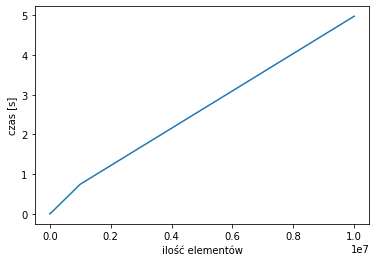
\includegraphics[width=0.8\linewidth]{wsi_1.png}
    \caption{Czas wykonania metody heurystycznej w funkcji ilości elementów}
\end{figure}

\begin{figure}[!h]
    \centering 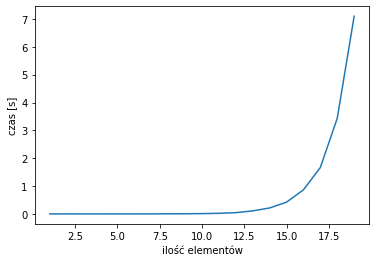
\includegraphics[width=0.8\linewidth]{wsi_2.png}
    \caption{Czas wykonania metody optymalnej w funkcji ilości elementów}
\end{figure}

\end{document}
